% topic4.tex -- Topic 4: Applications of the motor effect, Q55-72.
\topictitle{Topic 4 - Applications of the Motor Effect}

% ---- Q55 (torque on a motor coil)
\begin{quizq}{}
The coil of a DC motor has 100 turns, each of area \qty{0.010}{m^2}, and carries a current of
\qty{2.0}{A}. It is in a uniform magnetic field of \qty{0.20}{T}, with the plane of the coil parallel to
the field. What is the torque on the coil?
\opts{\qty{0}{N.m}}{\qty{0.0040}{N.m}}{\qty{0.20}{N.m}}{\qty{0.40}{N.m}}
\end{quizq}

% ---- Q56 (force and torque as the coil turns)
\Needspace{16\baselineskip}
\begin{quizq}{}
The coil of a DC motor starts with its plane parallel to a uniform magnetic field. The coil then
turns until its plane is at \ang{60} to the field. The current stays the same. Compared with the
start, what has happened to the force on each long side of the coil and to the torque on the coil?
\opts{The force on each side and the torque have both decreased.}
  {The force on each side is the same, but the torque has decreased.}
  {The force on each side and the torque are both the same.}
  {The force on each side has decreased, but the torque is the same.}
\end{quizq}

% ---- Q57 (split-ring commutator)
\Needspace{15\baselineskip}
\begin{quizq}{}
What is the function of the split-ring commutator in a DC motor?
\opts{It changes the AC supply into DC.}{It increases the strength of the magnetic field.}
  {It reverses the current in the coil every half turn, so the torque keeps acting in the same
   direction.}
  {It reduces the friction between the brushes and the coil.}
\end{quizq}

% ---- Q58 (back emf against angular velocity)
\Needspace{30\baselineskip}
\begin{quizq}{}
Which graph best shows how the back emf of a DC motor depends on its angular velocity $\omega$?
\gridopts{%
  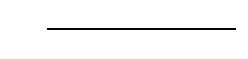
\begin{tikzpicture}\gaxesP{Back emf}{$\omega$}
    \draw[line width=1pt] (0,0.9) -- (2.4,0.9);
  \end{tikzpicture}}
  {%
  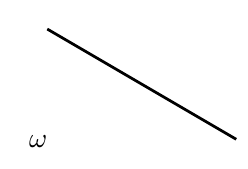
\begin{tikzpicture}\gaxesP{Back emf}{$\omega$}
    \draw[line width=1pt] (0,1.5) -- (2.4,0.1);
  \end{tikzpicture}}
  {%
  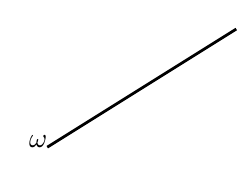
\begin{tikzpicture}\gaxesP{Back emf}{$\omega$}
    \draw[line width=1pt] (0,0) -- (2.4,1.5);
  \end{tikzpicture}}
  {%
  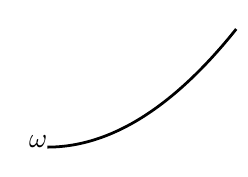
\begin{tikzpicture}\gaxesP{Back emf}{$\omega$}
    \draw[line width=1pt, domain=0:2.4, samples=30, smooth] plot (\x, {1.5*(\x/2.4)^2});
  \end{tikzpicture}}
\end{quizq}

% ---- Q59 (motor slowed by a load)
\Needspace{20\baselineskip}
\begin{quizq}{}
A DC motor is running at a steady speed. A heavier load is then attached, and the motor slows down.
Which row of the table describes the changes?
\begin{center}
  \renewcommand\arraystretch{1.7}
  \begin{tabular}{@{}p{10mm}|>{\centering\arraybackslash}p{50mm}|>{\centering\arraybackslash}p{50mm}|}
    \cline{2-3}
    & \textit{Back emf} & \textit{Current in the coil}\\ \cline{2-3}
    A. & Decreases & Increases\\ \cline{2-3}
    B. & Decreases & Decreases\\ \cline{2-3}
    C. & Increases & Increases\\ \cline{2-3}
    D. & Increases & Decreases\\ \cline{2-3}
  \end{tabular}
\end{center}
\end{quizq}

% ---- Q60 (back emf calculation)
\Needspace{12\baselineskip}
\begin{quizq}{}
A DC motor is connected to a \qty{24}{V} supply. Its coil has a resistance of \qty{2.0}{\ohm}. When the
motor runs at a steady speed, the current is \qty{1.5}{A}. What is the back emf?
\opts{\qty{3.0}{V}}{\qty{21}{V}}{\qty{24}{V}}{\qty{27}{V}}
\end{quizq}

% ---- Q61 (part not needed in an AC induction motor)
\Needspace{12\baselineskip}
\begin{quizq}{}
Which part is NOT needed in an AC induction motor?
\opts{Brushes and a commutator}{Stator coils}{A rotor (such as a squirrel cage)}{An AC supply}
\end{quizq}

% ---- Q62 (why the rotor turns slower than the field)
\Needspace{16\baselineskip}
\begin{quizq}{}
In an AC induction motor, the rotor always turns a little more slowly than the rotating magnetic
field of the stator. Why?
\opts{The rotor is too heavy to keep up with the field.}{Friction in the bearings slows the rotor.}
  {If the rotor turned as fast as the field, there would be no relative motion, so no current would be
   induced in the rotor and no torque would act.}
  {The rotating field reverses its direction too quickly for the rotor to follow.}
\end{quizq}

% ---- Q63 (output of a DC generator)
\Needspace{30\baselineskip}
\begin{quizq}{}
A coil rotates at a constant rate in a uniform magnetic field. It is connected to the external
circuit through a split-ring commutator. Which graph best shows the output voltage against time?
\gridopts{%
  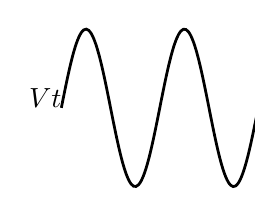
\begin{tikzpicture}\gaxesPN{$V$}{$t$}
    \draw[line width=1pt, domain=0:2.5, samples=80, smooth] plot (\x, {sin(288*\x)});
  \end{tikzpicture}}
  {%
  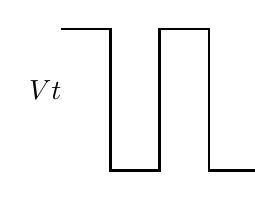
\begin{tikzpicture}\gaxesPN{$V$}{$t$}
    \draw[line width=1pt] (0,0.9) -- (0.625,0.9) -- (0.625,-0.9) -- (1.25,-0.9) -- (1.25,0.9) -- (1.875,0.9) -- (1.875,-0.9) -- (2.5,-0.9);
  \end{tikzpicture}}
  {%
  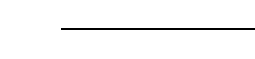
\begin{tikzpicture}\gaxesPN{$V$}{$t$}
    \draw[line width=1pt] (0,0.9) -- (2.5,0.9);
  \end{tikzpicture}}
  {%
  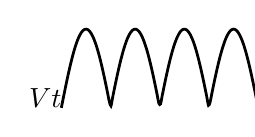
\begin{tikzpicture}\gaxesPN{$V$}{$t$}
    \draw[line width=1pt, domain=0:2.5, samples=120, smooth] plot (\x, {abs(sin(288*\x))});
  \end{tikzpicture}}
\end{quizq}

% ---- Q64 (generator turned twice as fast)
\Needspace{20\baselineskip}
\begin{quizq}{}
An AC generator is turned twice as fast. Which row of the table describes the change in its output?
\begin{center}
  \renewcommand\arraystretch{1.7}
  \begin{tabular}{@{}p{10mm}|>{\centering\arraybackslash}p{50mm}|>{\centering\arraybackslash}p{50mm}|}
    \cline{2-3}
    & \textit{Peak emf} & \textit{Frequency}\\ \cline{2-3}
    A. & Doubled & Doubled\\ \cline{2-3}
    B. & Unchanged & Doubled\\ \cline{2-3}
    C. & Doubled & Unchanged\\ \cline{2-3}
    D. & Halved & Doubled\\ \cline{2-3}
  \end{tabular}
\end{center}
\end{quizq}

% ---- Q65 (hand generator: hardest to turn)
\Needspace{14\baselineskip}
\begin{quizq}{}
A hand-turned generator is used to light identical bulbs. In which case is it hardest to turn the
generator at the same speed?
\opts{When nothing is connected to the generator}{When two bulbs are connected in series}
  {When one bulb is connected}{When two bulbs are connected in parallel}
\end{quizq}

% ---- Q66 (magnetic braking)
\Needspace{16\baselineskip}
\begin{quizq}{}
Some trains use magnetic braking: strong magnets on the train induce eddy currents in the metal rails.
Which statement about magnetic braking is correct?
\opts{The braking force is greatest when the train is moving slowly.}
  {The magnets must touch the rails to slow the train down.}
  {The eddy currents turn the train's kinetic energy into heat, and the braking force decreases as the
   train slows down.}
  {Magnetic braking can bring the train to a complete stop by itself.}
\end{quizq}

% ---- Q67 (Lenz's law and conservation of energy)
\Needspace{16\baselineskip}
\begin{quizq}{}
Which statement best explains how Lenz's law follows from the law of conservation of energy?
\opts{The induced current must be as large as possible, so that no energy is wasted.}
  {If the induced current helped the change that caused it, the change would keep growing, and energy
   would be created from nothing.}
  {The induced emf is always equal to the supply voltage.}
  {Energy is conserved only when the induced current is zero.}
\end{quizq}

% ---- Q68 (solid and slotted pendulums)
\Needspace{16\baselineskip}
\begin{quizq}{}
Two copper pendulum plates of the same size swing between the poles of a strong magnet. One plate is
solid. The other has several slots cut into it. Which statement is correct?
\opts{The slotted plate swings for longer, because the slots reduce the eddy currents.}
  {The solid plate swings for longer, because it has more mass.}
  {Both plates stop at the same time, because they are made of the same metal.}
  {The slotted plate stops sooner, because the slots increase the eddy currents.}
\end{quizq}

% ---- Q69 (efficiency of a motor)
\Needspace{12\baselineskip}
\begin{quizq}{}
A DC motor draws \qty{2.5}{A} from a \qty{12}{V} supply. It lifts a \qty{1.5}{kg} mass at a constant
speed of \qty{1.2}{m.s^{-1}}. What is the efficiency of the motor?
\opts{41\%}{59\%}{100\%}{170\%}
\end{quizq}

% ---- Q70 (average emf of a generator coil over a quarter turn)
\Needspace{13\baselineskip}
\begin{quizq}{}
A generator coil of 50 turns, each of area \qty{0.020}{m^2}, is in a uniform field of \qty{0.40}{T}. It
turns from a position at right angles to the field (maximum flux) to a position parallel to the field
(zero flux) in \qty{0.025}{s}. What is the average emf during this quarter turn?
\opts{\qty{0.32}{V}}{\qty{8.0}{V}}{\qty{16}{V}}{\qty{800}{V}}
\end{quizq}

% ---- Q71 (motors and generators)
\Needspace{16\baselineskip}
\begin{quizq}{}
Which statement about DC motors and generators is correct?
\opts{A motor changes mechanical energy into electrical energy.}
  {A generator needs a battery connected to it before it can produce a current.}
  {A motor and a generator use completely different parts.}
  {A generator changes mechanical energy into electrical energy, and a turning motor also acts as a
   generator, producing a back emf.}
\end{quizq}

% ---- Q72 (magnet swept past a copper block)
\Needspace{16\baselineskip}
\begin{quizq}{}
A strong magnet is moved quickly past a copper block that rests on a frictionless surface. What
happens to the block?
\opts{Nothing, because copper is not a magnetic material.}
  {It is pushed in the same direction as the magnet is moving.}
  {It is pushed in the opposite direction to the magnet's motion.}
  {It is attracted to the magnet and sticks to it.}
\end{quizq}
